\appendix

\chapter[Glossary of mechanical terms]{Glossary of \\ mechanical terms\label{app:Glossary}}

Here we list some definitions and concepts related to the terminology used in materials science and employed in \autoref{ch:Introduction}. A more comprehensive introduction to these terms can be found in \cite{ashby2005materials}.

\section*{List of definitions}

\begin{figure}[h!] 
\centering 
\includegraphics[scale=0.6]{TensileYield.pdf} 
\caption{Schematic of a tensile deformation experiment (left) and two possible forms of stress-strain curves. $\sigma_{zz}$ is equal to $F/A$. The blue curve represents the behavior of a \emph{brittle} sample, i.e. a sample that ruptures soon after that the stress-strain curve has deviated from linearity. The red curve represents the stress-strain curve of a \emph{ductile} sample, i.e. of a sample that can sustain tensile stress for large values of the deformation $\gamma$. In particular, the red curve shows \emph{work-softening}, with the sample sustaining less force as it is deformed at large strains. The slope of the dashed lines is the Young modulus $E$ of the sample associated to the red curve, and can be used to determine the 0.002 yield strain $\gamma_{y}$ and the yield stress $\sigma_{f}$ via the construction shown in the figure. The yield strain and stress ($\gamma_{y}$, $\sigma_{f}$) are the coordinates of the point where the line of slope $E$ passing through the point (0.002, 0) intercepts the stress-strain curve. \label{fig:AxialLoading}}
\end{figure}

\clearpage

For small deformation of a material in a tensile experiment (see \autoref{fig:AxialLoading}) the material behaves \emph{elastically}, i.e. $\sigma_{xx}$ shows a linear dependence from $\gamma$. We define the \emph{Young modulus} $E$ as
\begin{equation}
	E = \frac{\sigma_{zz}}{\gamma}
\end{equation}
where $\sigma_{zz}$ is the value of stress in the direction of the loading corresponding to a deformation $\gamma$ measured in the linear part of the stress-strain curve (see \autoref{fig:AxialLoading}).
$E$ is thus the slope of the stress-strain curve in an interval close to the origin.

The \emph{strength} $\sigma_{f}$ is defined for metals as the value of the stress at which the stress-strain curve for axial loading (see \autoref{fig:AxialLoading}) deviates by a strain of 0.002 from the linear elastic line.

The \emph{yield strain} $\gamma_{y}$ is the value of strain at which the stress-strain curve assumes the value $\sigma_{f}$ (see \autoref{fig:AxialLoading}). It is thus the value of the strain at which the sample ceases to be linearly elastic upon axial loading, where the exact definition of ``ceasing to be elastic'' depends on the definition of $\sigma_{f}$. 

The \emph{hardness} $H$ is the quantity measured by pressing a pyramid-shaped indenter onto the surface of a material and is expressed by the formula
\begin{equation}
	H = \frac{P}{A}
\end{equation}
where $P$ is the load (force) applied on the indenter and $A$ is the area of the base of the pyramid-shaped indent caused on the surface (see \autoref{fig:Hardness}). Hardness is related to strength $\sigma_{f}$ by the approximate relationship $H = 3\sigma_{f}$.

\begin{figure}[h!] 
	\centering 
	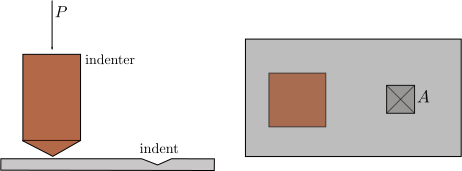
\includegraphics[width=0.8\textwidth]{Indenter.pdf} 
	\caption{Schematic side (left) and top (right) view of an indentation experiment to obtain the hardness of a material. \label{fig:Hardness}}
\end{figure}

The \emph{resilience} is the area under the stress-strain curve up to $\gamma = \gamma_{y}$ (see \autoref{fig:Resilience}):
\begin{equation}
	\text{resilience} = \int_{0}^{\gamma_{y}} \sigma_{zz} d\gamma
	\label{eq:Resilience}
\end{equation}
Materials with a high resilience are able to store elastically large quantities of energy.

\begin{figure}[h!] 
\centering 
\includegraphics[scale=0.6]{Resilience.pdf} 
\caption{Stress-strain curve in an experiment where the sample is subjected to tensile loading. The shaded area represents the resilience in \autoref{eq:Resilience}. \label{fig:Resilience}}
\end{figure}

The \emph{loss coefficient} is defined as the ratio
\begin{equation}
	\eta =  \frac{\oint \sigma_{zz} d\gamma}{\int_{0}^{\gamma_{max}} \sigma_{zz} d\gamma}
	\label{eq:LossCoefficient}
\end{equation}
which is the ratio of the area of the hysteresis loop when a material is deformed cyclically up to some value $\gamma_{max}$ and the amount of energy stored in the system when it is deformed up to $\gamma_{max}$ (\autoref{fig:LossCoefficient}). The loss coefficient is also the inverse of the $Q$ factor for a mechanical oscillator \cite{ashby2005materials}.

\begin{figure}[h!] 
\centering 
\includegraphics[scale=0.6]{LossCoefficient.pdf} 
\caption{Hysteresis stress-strain curve in an experiment where the sample is loaded cyclically. The loss coefficient in \autoref{eq:LossCoefficient} is the ratio between the value of the red area and the light blue one. \label{fig:LossCoefficient}}
\end{figure}

\chapter{The mortal random walk \label{app:MortalRandomWalk}}

\section*{Derivation of the expression of the MSD}

A particle system formed by $N$ particles undergoing deformation can be represented as a state point in the $3N$-dimensional coordinate space. 
Here we focus on the configurations visited by a system subjected to oscillatory deformation at $\gamma = 0$, and assume that systems during such an experiment can be in two states:
\begin{itemize}
	\item they're diffusing (``alive''), with a certain diffusion constant $D$ (they thus perform a random walk in configuration space). On average, they move farther and farther from the configuration assumed for $\gamma_{acc} = 0$ as $\gamma_{acc}$ increases;
	\item they're absorbing (``dead''), and retain their coordinates for arbitrarily large values of $\gamma_{acc}$.
\end{itemize}
Furthermore, we assume that systems diffusing under deformation have some finite probability $\lambda$ per unit $\gamma_{acc}$ to stop their diffusive motion, thus becoming absorbing. Such ``mortal'' dynamics clearly violates the principle of detailed balance\footnote{Detailed balance is violated because a ``living'' state can ``die'', whereas resurrections are not possible!}. \\

The probability $P(r, \gamma_{acc})$ to find a configuration at a distance $r = \sqrt{N \cdot \text{MSD}}$ away from the starting point where the system is at $\gamma_{acc} = 0$ after an oscillatory deformation of $\gamma_{acc}$ is given by:
\begin{align}
	P(r, \gamma_{acc}) 	&= P_{alive}(r, \gamma_{acc}) + P_{dead}(r, \gamma_{acc}) \\
						&= P_{alive}(\gamma_{acc}) P_{RW}(r,\gamma_{acc}) + \sum_{\gamma_{acc}'} P_{dying}(\gamma_{acc}') P_{RW}(r,\gamma_{acc}') \\
						&= P_{alive}(\gamma_{acc}) P_{RW}(r,\gamma_{acc}) + \sum_{\gamma_{acc}'} P_{alive}(\gamma_{acc}') \lambda\ P_{RW}(r,\gamma_{acc}') \\
						&\approx e^{-\lambda \gamma_{acc}} P_{RW}(r,\gamma_{acc}) + \int_{0}^{\gamma_{acc}} d\gamma_{acc}'\ e^{-\lambda \gamma_{acc}'} \lambda\ P_{RW}(r,\gamma_{acc}')
\end{align}

where $P_{RW}(r, \gamma_{acc})$ is the probability for a random walker to be at a distance $r$ away from the starting point after a deformation on $\gamma_{acc}$.
As the mean squared displacement is defined as the second moment of $P(r,\gamma_{acc})$, we have 
\begin{align}
	\text{MSD}(\gamma_{acc})	&= \frac{1}{N} \int dr\ r^{2} P(r,\gamma_{acc}) = \langle r^{2}(\gamma_{acc}) \rangle \\
								&= \frac{1}{N}\, e^{-\lambda \gamma_{acc}} D \gamma_{acc} + \frac{1}{N}\, \int_{0}^{\gamma_{acc}} d\gamma_{acc}'\ e^{-\lambda \gamma_{acc}'} \lambda\ D \gamma_{acc}' \\
								&= \frac{D}{\lambda N} (1 - e^{-\lambda \gamma_{acc}})
\end{align}
where the solution is obtained by integrating by parts and imposing $\text{MSD}(0) = 0$ as a boundary condition. This expression of the mean squared displacement is used to fit the diffusion behavior in \autoref{sec:DiffusionBehavior}.

\chapter{Details of the NK model \label{app:NKDetails}}

\section*{Reduction of the allowed configuration space}

In \autoref{sec:NKModel} the set of the configurations accessible to the NK models is restricted to the subset of $N$-tuples formed by ones and zeros that have the following property:
\begin{equation}
    \sum_{i} m_{i} = \frac{N}{2}
    \label{eq:NKConstraint}
\end{equation}

The reason to use this configuration space rather than the set of the $2^{N}$ $N$-tuples formed by ones and zeros is a bit subtle, and can be understood by looking at the following example. 
If the $a$ function in \autoref{eq:NKCouplings} is such that
\begin{equation}
    \{0, \ldots, 0\} \xrightarrow{a} \frac{1}{4}
    \label{eq:PathologicNKCoupling}
\end{equation}

(so that the $(K+1)$-tuple formed by zeros only maps through $a$ onto $\frac{1}{4}$) the value of the energy as measured from \autoref{eq:NKEnergy} yields, for the configuration where all the $N$ spins are identically zero, when $\gamma$ = 0:
\begin{align}
    E   &= -\frac{1}{2} \sum_{i = 1}^{N} \left( 1 + \sin(2 \pi a_{i} + \gamma b_{i} \right)) \notag \\
        &= -\frac{1}{2} \sum_{i = 1}^{N} \left( 1 + 1 \right) = - N
    \label{eq:PathologicNKEnergy}
\end{align} 

so that the energy assumes the lowest possible value ($- N$) in correspondence of the configuration where all spins are $0$. The sum in \autoref{eq:PathologicNKEnergy} gets simplified because all spins are equal to zero, all their neighbors are zero too, and thus each term $a_{i} = \frac{1}{4}$ for all $i$. The value that the map $a$ assumes in correspondence with the null $(K+1)$-tuple gives rise to a very deep energy ground state (which is the null $N$-tuple), and neighboring configurations will (in general) have an energy strictly higher, analogously to what happens in the case of ferromagnetic states in the Ising model. 
The presence of a such a deep inherent structure in the NK landscape poses a problem because its basin is a potentially vast ``funnel'' that easily attracts the system during AQS dynamics\footnote{Loosely speaking, the ``ferromagnetic'' configuration acts as a crystalline configuration which can be easily reached starting from any point of the energy landscape.}. Furthermore, by changing $\gamma$ such a deep minimum is possibly not destabilized, especially if $b$ in \autoref{eq:NKCouplings} maps the null $(K+1)$-tuple to a value close to 0.\\
The same problem of course exists if $a$ maps the $K$-tuple formed by all ones onto a value close to $1/4$. 
Two strategies can be envisaged in order to cure this problem:

\begin{enumerate}
    \item restricting the possible values of the couplings $a$ and $b$: the ``pathologic'' values of the couplings $a$ and $b$ can be forced not to assume problematic values in correspondence to the $(K+1)$-tuples with all equal values. This can achieved in practice by choosing a non-uniform probability distribution in the choice of the values of the couplings \autoref{eq:NKCouplings}. This presumably rules out energy landscapes presenting ``trivial'' deep ground states and undesired topologies. It's not clear, however, what kind of probability distribution one should use;
    \item restricting the number of states: the problematic states of the energy landscape can simply be removed from the accessible landscape. This is the choice made in \autoref{sec:NKModel} and summarized by \autoref{eq:NKConstraint}, where just the subset of all the $N$-tuples of constant ``magnetization'' equal to $N/2$ is taken as the set of allowed configurations. Such method is arguably more elegant than the previous one, but comes at a high price: whereas in the entire space of the $N$-tuples configurations lie on a simple (hyper-)cubic lattice where all configurations have $N$ nearest neighbors at a distance $d=1$, in the subset nearest neighbors are separated by $\sqrt{2}$ and are many more ($N^{2}/4$). This increases the complexity of the steepest descent algorithm used to perform AQS on the NK model, making the study of the model computationally expensive if $N$ is large.
\end{enumerate}

\section*{Example of the NK model, ground state degeneracy}

A simple example can help to understand how the NK model works, and some of the features that it can have (in this case, ground state degeneracy). We set $\gamma=0$ for simplicity and take $N = 4, K = 1$:
Consider the map $a$:
\begin{equation}
	\{0, 0\} \xrightarrow{a} 0 \quad 
	\{0, 1\} \xrightarrow{a} \frac{1}{4} \quad
	\{1, 0\} \xrightarrow{a} 0 \quad
	\{1, 1\} \xrightarrow{a} 0 \quad{}
	\label{eq:NKExampleCouplings}
\end{equation}

and the neighbor lists for each spin:
\begin{equation}
	\{1, 2\}, \{2, 1\}, \{3, 4\}, \{4, 3\}
	\label{eq:NKExampleNeighbors}
\end{equation}

Let's enumerate all the energies of the allowed 4-tuples, calculated from the expression in \autoref{eq:NKEnergy} using the information in \autoref{eq:NKExampleCouplings} and \autoref{eq:NKExampleNeighbors}: 
\begin{align}
	E (0, 0, 1, 1) = -2 \notag \\
	E (0, 1, 0, 1) = -3 \notag \\
	E (0, 1, 1, 0) = -3 \notag \\
	E (1, 0, 0, 1) = -3 \notag \\
	E (1, 0, 1, 0) = -3 \notag \\
	E (1, 1, 0, 0) = -2 
\end{align}

In this simple example one sees that the minimum possible value of energy $-N = -4$ is not attained and that the ground state is four-fold degenerate.

\section*{Density of states and of inherent structures in the NK model}

A distinctive and nice feature of the NK model is that it has a discrete set of states: for a given value of $N$ there are $\binom{N}{N/2}$ allowed configurations. If this number is not too large one can enumerate each of them and calculate their energy by means of \autoref{eq:NKEnergy}. In this way one can calculate the density of states (DOS). This is done in \autoref{fig:NKDensityOfStates}, where the density of states is shown to be gaussian. 

\begin{figure} 
\centering 
\includegraphics[width=0.8\textwidth]{MapNK20.pdf} 
\caption{Density of states and of inherent states of an NK model with $N=20$ and $K=10$. The form of the DOS is gaussian. \label{fig:NKDensityOfStates}}
\end{figure}

Furthermore, by applying a steepest descent (SD) procedure using Kawasaki moves \cite{domb2000phase}, one can even \emph{minimize all the allowed states one by one} (at least if $N$ is small enough), and thus find \emph{all} the inherent structures of the NK landscape and their energies. This brute force approach is clearly not feasible with particle systems, where the set of allowed states is not countable. Doing so, one can extract the density of inherent states, which is also plotted in \autoref{fig:NKDensityOfStates}. Clearly, the features of the DOS mentioned above will depend on the choice of $N$, $K$, and the value of the parameters needed to compute $E$ in \autoref{eq:NKEnergy}.
Whenever brute force computation of the states is feasible, the system can be studied at some given $T$ by calculating the partition function via the sum of the Boltzmann factors $e^{-\beta U}$, and ensemble averages can be performed in a straightforward way. If $N$ is large, however, the number of states becomes huge, and the system needs to be studied by means of sampling methods, like the Monte Carlo method \cite{frenkel2001understanding}. To do this one starts from some given configuration and attempts Kawasaki moves to neighboring ones, accepting or rejecting the moves according to the Metropolis rule for the given $T$. After a transient, the system equilibrates on a trajectory that samples states with a probability proportional to their Boltzmann factor. Such states can be minimized in energy via SD so to obtain the associated inherent structures, which in turn can be used as starting configurations for athermal ``deformation'' simulations.

\chapter{Details of the TM model \label{app:TMDetails}}

\section*{Details of the construction of $P$}

Here we describe how the assumptions listed in \autoref{sec:TMAssumptions} can be used to construct $P$.
First of all, one can see that
\begin{equation}
    P = P_{-} P_{+} 
\end{equation}
so that the construction of $P$ is reduced to that $P_{+}$ and $P_{-}$. 
Each of these (say $P_{+}$), can in turn be viewed as the composition of matrices 
\begin{equation}
P_{+} =
P_{\leftarrow}^{0}
\ldots
P_{\leftarrow}^{\gamma_{max} - d\gamma}
P_{\rightarrow}^{\gamma_{max}}
P_{\rightarrow}^{\gamma_{max} - d\gamma}
\ldots
P_{\rightarrow}^{2d\gamma}
P_{\rightarrow}^{d\gamma}
\end{equation}

where $P_{\rightarrow}^{\gamma^{*}}$ is the matrix describing how AQS dynamics maps the inherent structures of the landscape relative to $\gamma = \gamma^{*} - d\gamma$ into the set of the structures of the landscape associated to $\gamma = \gamma^{*}$. The arrows in the subscript indicate whether $P^{\gamma^{*}}$ is associated to an increase of $\gamma$ ($\rightarrow$) or a decrease ($\leftarrow$) in strain. For instance, $P_{\leftarrow}^{\gamma^{*}}$ describes how AQS maps the structures of the $\gamma = \gamma^{*} + d\gamma$ landscape onto those associated to $\gamma = \gamma^{*}$. 
As the landscape is assumed to have $M$ inherent structures no matter the value of $\gamma$, each of these $P_{\rightarrow}^{\gamma^{*}}$, $P_{\leftarrow}^{\gamma^{*}}$ is a square matrix.
To construct each of the $P_{\rightarrow}^{\gamma^{*}}$ one uses the assumption that the probability per unit strain to destabilize a given inherent structure is equal to $\tau$. So, when the strain is incremented by $d\gamma$, a system in a given inherent structure has probability $1 - \tau d\gamma$ to be in a structure $i$ that is not destabilized, and thus it maps to the same structure $\mathbf{R_i}$ in the deformed landscape through $P_{\rightarrow}^{\gamma^{*}}$. In that case the matrix element $P_{\rightarrow, ii}^{\gamma^{*}} = 1$. The system has also a probability $\tau d\gamma$ to be in a structure $\mathbf{R_j}$ that is destabilized by the strain increment, so that it falls onto some randomly chosen inherent structure $\mathbf{R_k}$ of the deformed landscape. in that case the matrix element $P_{\rightarrow, kj}^{\gamma^{*}} = 1$. Incidentally, for each configuration $\mathbf{R_l}$ that is destabilized at $\gamma^{*}$ as strain is increased, another configuration $\mathbf{R_m}$ is correspondingly created at that strain value. This means that $\mathbf{R_m}$ will be destroyed at $\gamma^{*}$ when the strain will be decreased (due to the symmetry of the landscapes). This is a constraint on the form of the matrix $P_{\leftarrow}^{\gamma^{*}}$: $P_{\leftarrow}^{\gamma^{*}}$ must be constructed by taking into account that the structures that are destroyed at $\gamma^{*}$ when incrementing $\gamma$ are exactly those created at $\gamma^{*}$ when decrementing $\gamma$.\\
The procedure outlined above is used to create a matrix $P_{+}$ associated to some $\gamma_{max}$. The $P_{+}'$ corresponding to another $\gamma_{max}'$ is simply given by 
\begin{align}
P_{+}' = &
P_{\leftarrow}^{0}
\ldots
P_{\leftarrow}^{\gamma_{max}' - d\gamma}
P_{\rightarrow}^{\gamma_{max}'}
P_{\rightarrow}^{\gamma_{max}' - d\gamma}
\ldots
P_{\rightarrow}^{2d\gamma}
P_{\rightarrow}^{d\gamma} 
\quad \text{if } \gamma_{max}' < \gamma_{max} \\
P_{+}' = &
P_{\leftarrow}^{0}
\ldots
P_{\leftarrow}^{\gamma_{max} - d\gamma}
P_{\leftarrow}^{\gamma_{max}}
P_{\leftarrow}^{\gamma_{max} + d\gamma}
\ldots
P_{\leftarrow}^{\gamma_{max}' - d\gamma}
P_{\rightarrow}^{\gamma_{max}'} 
P_{\rightarrow}^{\gamma_{max}' - d\gamma} \notag\\
&
\ldots 
P_{\rightarrow}^{\gamma_{max} + d\gamma}
P_{\rightarrow}^{\gamma_{max}}
P_{\rightarrow}^{\gamma_{max} - d\gamma}
\ldots
P_{\rightarrow}^{2d\gamma}
P_{\rightarrow}^{d\gamma} 
\quad \text{if } \gamma_{max}' > \gamma_{max} 
\end{align}

Using this procedure its thus possible to create a sequence of matrices relative to multiple values of $\gamma_{max}$.

A Python code capable of generating $P_{+}$ (or $P_{-}$) for a given value of $\gamma_{max}$ is proposed below.

\section*{Python implementation}

Here we quote some Python code capable of generating one of the $P_{+}$ and $P_{-}$ matrices using the assumptions of the TM model. We warn the reader that this is a short and readable implementation that is not efficient as the size of the matrices $M$ gets large. For large $M$, sparse matrices need to be employed (these can be easily handled by the SciPy library \cite{scipy}).   

\begin{quote}
\small
    \VerbatimInput[numbers = left]{main/createP.py}
    \normalsize
\end{quote}

\chapter[Athermal deformation of gels and bigels]{Athermal deformation \\ of gels and bigels \label{app:Gels}}

In this appendix, after a brief description of their properties, we discuss how \emph{particle gels} and \emph{bigels} (a new kind of system recently found in computer simulations and realized experimentally using DNA-coated colloids \cite{varrato2012arrested}) behave under athermal quasi static deformation. Even though these systems are physically different from metallic glasses, a qualitative treatment of their properties can be performed using the same methods that have been described in \autoref{ch:ParticleModels} and employed in \autoref{ch:ParticleModelsResults}, with minor modifications to the model. 
The main findings presented in this chapter have been published in \cite{dimichele2013aggregation}.

\section*{Gels and bigels}

If a fluid above its critical temperature is cooled down and crosses its gas-liquid transition line, it separates in two distinct phases in equilibrium. Such phases coexist at the same pressure, and have different densities.
A particular example is constituted by \emph{colloids}. In a colloid, solid particles (named \emph{colloidal particles}) whose size ranges from $\SI{1}{\nano\metre}$ to $\SI{1}{\micro\metre}$ are dispersed in a liquid solvent\footnote{In an experimental setup the density of the colloidal particles is often made equal to that of the solvent, so that the effect of gravity is compensated by buoyancy.}. Above some critical temperature the colloidal particles form a single homogeneous phase. If the system is cooled down (or, conversely, the interactions between the particles are strengthened) the system can separate in a ``colloid-rich'' phase (which is characterized by a high density of colloidal particles) and a ``colloid-poor'' one, separated by an interface. The dynamics of such phase separation depends on the nature of the system and on the rate at which the system is cooled down. One of the ways in which the system can separate in two phases goes under the name of \emph{spinodal decomposition}. In a spinodal decomposition phase separation takes place everywhere in a given sample, with the two phases organizing in an intertwined structure whose characteristic lengthscale grows with time.
For some kinds of interparticle interactions, if the quench is sufficiently fast so that low temperatures are reached before such lengthscale has grown, the spinodal decomposition can be \emph{arrested} \cite{foffi2005scaling, foffi2005arrested, lu2008gelation}. This arrest is similar to the one observed in glasses, with the system maintaining for long times configurations out of equilibrium, rather than separating into two bulk phases separated by an interface. The arrested configuration observed in some colloidal systems is an inhomogeneous, ramified, tenuous and system spanning structure composed of colloidal particles, which goes under the name of \emph{particle gel}. Particle gels have been observed for instance in \cite{lu2008gelation}, using colloids formed by PMMA beads suspended in a solvent with the same density and refractive index of the beads. In that case the ``quench'' is obtained by adding linear polystyrene chains to the solution, so to induce an effective isotropic depletion attraction \cite{likos2001effective} between the particles.
Qualitatively, similar results have been obtained in MD simulations modeling colloids as point particles interacting via the Asakura-Oosawa potential (which is the analytical description of depletion interaction \cite{likos2001effective}) or a modified Lennard-Jones potential characterized by a very short interaction range\cite{lu2008gelation}, as well as in event-driven MD of point particles interacting via a short-ranged square-well potential. \\
Recently, a more complex class of systems was discovered \cite{varrato2012arrested}, by using mixtures of particles as those described above, characterized by an attractive interaction between particles of the same species and a repulsive interaction between particles of different species. Systems of this kind could be realized experimentally by grafting polystyrene beads with functionalized DNA, which is able to induce attraction on complementary strands. As these systems are quenched by lowering the temperature, the mixture undergoes \emph{demixing} \cite{dorsaz2010phase} and finally colloidal particles form interpenetrating structures. Each of of these structures is composed by particles of a single species only, and is very close to that of a gel. In the case of binary mixtures, these structures were named \emph{bigels} \cite{varrato2012arrested}.
Similar structures have been first obtained by means of event driven MD simulations \cite{varrato2012arrested}, quenching particles interacting with an intraspecies square-well potential and a hard-sphere interspecies potential. 

\section*{Computer simulation of gels}

The mechanical properties of \emph{particle gels} are a subject of ongoing investigations (see \cite{rajaram2010microstructural, sprakel2011stress} for examples of recent experimental work), and those of bigels have (to our knowledge) never been probed before, neither in experiments nor simulations. In what follows we present computer simulations of AQS deformation of gel-like and bigel-like structures obtained by using a short-ranged Lennard-Jones potential.

\subsection*{Modified Lennard-Jones binary mixture}

In what follows we consider a modified cut and shifted Lennard-Jones potential of the form
\begin{equation}
	U_{\alpha \beta}(r) = 
	\left\{
	\begin{array}{rl}
			4 \epsilon \left( \left( \frac{\sigma}{r} \right)^{m} - \left( \frac{\sigma}{r} \right)^{n} \right) + U^{shift}_{\alpha \beta},	& \text{if }	r 		\le		\lambda_{\alpha \beta} \sigma		\\
			0,	& \text{if }	r 	> \lambda_{\alpha \beta} \sigma				\\
	\end{array}
	\right. ,
	\label{eq:ModifiedLennardJones}
\end{equation}
where $m = 64$, $n = 32$, in order to get a short ranged potential. We use this potential both to describe interaction within a pure fluid of a single species (so that its concentration is $c=N_{A}/N=1$) and a symmetric two-component mixture ($c=0.5$).
The choice of parameters here is $\epsilon = 1$ and $\sigma = 1$, and the attraction and repulsion is determined by the value of the cut-off $\lambda_{\alpha \beta}$. By setting $\lambda_{AB} = 1$ and $\lambda_{AA} = \lambda_{BB} = 1.4$ the interspecies interaction is made purely repulsive, whereas attraction exists at intermediate range for particles of the same species. The choice of the exponents is such to make the potential $U_{AB}$ sufficiently short-ranged, and $U_{shift}$ is chosen to make $U_{\alpha \beta}$ continuous at the cut-off.

\subsection*{Preparation of the samples}

We take a system composed by $N = 50000$ particles of species $A$ at packing fraction\footnote{If one assumes that the volume occupied by a single particle is equal to $\frac{4}{3} \pi \left(\frac{\sigma}{2}\right)^{3}$, the packing fraction $\phi$ is defined to be fraction of the overall volume occupied by the particles. The packing fraction is related to the number density $\rho$ through the formula $\phi = \frac{\pi}{6} \rho$ if $\sigma = 1$.} $\phi = 0.1$, and another one of the same dimensions composed by $N_{A} = 25000$ of species $1$ and $N_{B} = 25000$ of species $2$ and simulate it using LAMMPS\footnote{The potential in \autoref{eq:ModifiedLennardJones} is not implemented in LAMMPS for general values of $m$ and $n$, and was coded by the author following the templates available within the source code of LAMMPS (see \cite{mygithub}).}. Such particles are initially placed at random in a simulation box with periodic boundary conditions. Then, an energy minimization is applied in order to remove overlaps between the particles. 
The two systems are initially thermostated at $T=100$, and subsequently quenched from $T=100$ to $T=0.01$ by connecting them to a Berendsen \cite{hunenberger2005thermostat} thermostat at $T=0.01$. The initial temperature is chosen to have such a high value so to follow a procedure which is as close to that followed in \cite{varrato2012arrested} as possible. In order to ensure numerical stability at high temperatures, when particles have a high kinetic energy and thus undergo large displacements per unit time, a very small time step $dt = 10^{-5}$ (in reduced units) is employed. As the temperature is decreased, $dt$ is increased to $0.001$ to reduce computational overhead and follow the system for longer times.

\begin{figure}
	\centering
	\begin{subfigure}[b]{0.5\textheight}
		\centering
		\includegraphics[width = 0.5\textheight]{TVstGelBigel.pdf}
		\caption{\label{fig:TVstGelBigel}}	
	\end{subfigure}
	\begin{subfigure}[b]{0.5\textheight}
		\centering
		\includegraphics[width = 0.5\textheight]{UVstGelBigel.pdf}
		\caption{\label{fig:UVstGelBigel}}
	\end{subfigure}	
	\caption{(\subref{fig:TVstGelBigel}) Temperature profile applied over time during the quench of the single component and the two component mixture. (\subref{fig:UVstGelBigel}) Potential energy profile during the quench for the two cases. During the quench the energy progressively lowers, and finally reaches a regime where it drifts extremely slowly downward. At this stage ($t \approx 10^{3}$) the gel and bigel structures can be considered to be arrested. \label{fig:QuenchGelBigel}}
\end{figure}

The result of this preparation are respectively gel-like and bigel-like structures, whose visual inspection (see snapshots on the top \autoref{fig:GelBigelDeformation}) reveals a strong resemblance with what is observed in simulations using square well interaction potentials in \cite{varrato2012arrested}. In addition, after having waited enough time after the beginning of the quench, both the MSD of the particles and the potential energy $U$ (\autoref{fig:QuenchGelBigel}) saturate to nearly-constant values. At that stage, one can consider the phase separation to be arrested.

\pagebreak

\subsection*{Athermal deformation behavior of gels and bigels}

Quenched configurations that have reached a plateau in the potential energy and MSD are subjected to a potential energy minimization using the conjugate-gradient algorithm. This allows them to reach mechanically stable minima. Such configurations of minimum energy are shear-strained up to a large values of the strain ($\gamma = 10$) by varying the boundary conditions using the AQS procedure described in \autoref{ch:ParticleModels} and employing a $d\gamma = 10^{-5}$. Imposing energy minimization at each AQS step corresponds to considering the system as composed of ``sticky'' particles, able to form and destroy bonds only as a consequence of a change in strain.
Values of the shear stress in the plane of the applied strain and configurations are computed with \autoref{eq:StressTensorComponent} and dumped at regular intervals as the strain is increased, so that the evolution of the sample under deformation can be monitored. \\
The mechanical behavior of gels and bigels is very different, at least for the set of parameters chosen here. For low values of the strain, the two systems both show an elastic behavior with a linear dependence of the shear stress from the shear strain \autoref{fig:SigmaVsGammaGelBigel}. The bigel, however, appears to be much stiffer than the gel. This is possibly due to the fact that deformation brings different branches of the intertwined structure in contact, and that the two systems behave in a different way as a consequence of this. In the gel, branches brought in contact are formed by particles of the same species, and thus when in contact stick together because of the attractive intraspecies interaction. In a bigel, instead, branches in contact can be formed by particles belonging to different species. In this latter case, branches do repel each other, and thus impede the system to comply to the deformation.
At a larger value of the strain, which is approximately equal for the two kinds of systems, the stress deviates from linearity and both the gel and the bigel yield. As a consequence of the larger stiffness of the bigel, its yield stress is much larger than that of the gel. For strains larger still, the two systems undergo large modifications, but in qualitatively distinct ways (see \autoref{fig:GelBigelDeformation}). The ramified structure of the gel is gradually destroyed, with dangling branches lumping together so to form a less porous structure which is clearly not percolating in the simulation box, and a stress correspondingly falling to low values for large strains. Such compaction is not observed in the case of bigels. In fact, as strain is increased, the ramified structure of bigels breaks up into a ``gas'' of disconnected clusters of particles of the two species. Is this difference in behavior related to the fact that the two component of a bigel form structures that more tenuous than those of a gel with the same packing fraction? In principle this could be true, because the gel is a single structure made out of $N$ particles, whereas the bigel is made out of two intertwining networks each containing $N_{A} = N_{B} = N/2$ particles. We have verified that this is not the case by studying the deformation behavior of a single component gel formed by $N/2$ particles in a box with the same dimensions as that used with the gels with $N$ particles. This system is approximately equivalent to the structure formed by a single component in a bigel, if the one formed by the other component is disregarded. We checked that the large deformation behavior of such a gel (with $\phi = 0.05$) is qualitatively equivalent to that of the $\phi = 0.1$ gel.
This suggests that the difference in the large strain behavior observed in bigels is likely to be due to the presence of particles of the other species, which behaves like an obstacle that impedes to particles of a given species to bond together and form a large compact cluster.

\begin{figure}
	\centering
	\includegraphics[width = 0.7\textwidth]{SigmaVsGammaGelBigel.pdf}
	\caption{Shear stress as a function of shear strain averaged over $\approx 8$ gel and bigel samples of $\phi = 0.1$. The bigel is stiffer, and is able to sustain a larger stress for large values of the strain.\label{fig:SigmaVsGammaGelBigel}}
\end{figure}

\begin{figure}
	\centering
	\includegraphics[width = 0.4\textwidth]{gel-0.png}
	\includegraphics[width = 0.4\textwidth]{bigel-0.png} \\
	\includegraphics[width = 0.4\textwidth]{gel-1.png}
	\includegraphics[width = 0.4\textwidth]{bigel-1.png} \\
	\includegraphics[width = 0.4\textwidth]{gel-2.png}
	\includegraphics[width = 0.4\textwidth]{bigel-2.png} \\
	\includegraphics[width = 0.4\textwidth]{gel-8.png}
	\includegraphics[width = 0.4\textwidth]{bigel-8.png} \\
	\caption{Configuration of a gel (left) and a bigel (right) of $\phi = 0.1$ at $\gamma = 0, 1, 2, 8$. With an increase in shear strain, the gel ruptures and compacts. The bigel does form a gas of disconnected clusters instead. \label{fig:GelBigelDeformation}}
\end{figure}

\begin{landscape}

\begin{figure}
	\centering
	\begin{subfigure}[b]{0.5\textheight}
		\centering
		\includegraphics[width = 0.5\textheight]{ClusterGels-pf010.pdf}
		\caption{Gel at $\phi = 0.1$.}	
	\end{subfigure}
	\begin{subfigure}[b]{0.5\textheight}
		\centering
		\includegraphics[width = 0.5\textheight]{ClusterGels-pf005.pdf}
		\caption{Gel at $\phi = 0.05$.}
	\end{subfigure}	
	\begin{subfigure}[b]{0.5\textheight}
		\centering
		\includegraphics[width = 0.5\textheight]{ClusterBigels-pf010.pdf}
		\caption{Bigel at $\phi = 0.1$.}
	\end{subfigure}
	\caption{In these heatmaps, we represent the total number of particles of species $A$ that belong to a cluster whose size is indicated on the $y$-axis, as a function of the strain $\gamma$, for gels and bigels systems. Particles are considered to belong to the same cluster if they belong to the same species and their centers are separated by a distance lower than 1.4. Under deformation the particles of the gels form a single cluster containing almost all the particles (in the case of the gel at $\phi = 0.05$, the largest cluster actually \emph{grows}). In the case of the bigel, the structure breaks into smaller clusters as strain is increased. \label{fig:ClustersVsGammaGelBigel}}
\end{figure}

\end{landscape}

\subsection*{Summary and outlook}

Our data show that bigels have interesting mechanical properties that differentiate them from gel structures formed by particles of a given kind only. Gels and bigels are both elastic at small strains, but bigels appear stiffer. Large strains are able to destroy the percolating structures in both the cases of gels and bigels. However, gels and bigels do rupture in quite different ways, with gels aggregating is a single, dense cluster and bigels breaking up in multiple smaller clusters (at least in the range of strains examined here).
One can speculate, on the basis of our data, that a reversal of the strain will not make any of the two kinds of systems recover the ramified and percolating configurations that they had before the deformation. We posit that the result of strain reversal of deformed gels will be a compact cluster, and a gas of clusters in the case of bigels, with none of the two systems showing the capability to spontaneously heal as strain is reversed.\\
Our results could be confirmed by carrying out rheological experiments on bigels, with particle positions being able to be measured by means of confocal microscopy as in \cite{varrato2012arrested}.

\chapter{Data preservation \label{app:DataPreservation}}

Part of the data presented in the plots and the scripts needed to generate them are available together with code related to the LJ, NK, and TM models and the input parameters used in the simulations on\\

\centerline{\url{https://github.com/davidefiocco/phd-thesis}}

On this repository (referred to in the text as ``\cite{mygithub}'') the interested reader can find the additional material mentioned in the thesis and a list of corrections to typos.

